\documentclass[11pt]{article}
\usepackage[margin=1in]{geometry}
\usepackage[T1]{fontenc}
\usepackage{amsmath,amsthm}
\usepackage{newtxtext,newtxmath,microtype}
\usepackage{booktabs,graphicx,array,enumitem}
\usepackage[authoryear,round]{natbib}
\usepackage{xcolor}
\usepackage{xurl}
\usepackage[colorlinks=true,linkcolor=blue!40!black,citecolor=blue!40!black,urlcolor=blue!40!black]{hyperref}
\hypersetup{pdftitle={Who Can Move the Money? Delegated Deposit Control and Bank Liquidity},pdfauthor={Shivam Gupta},pdfsubject={Financial intermediation and delegated withdrawal authority},pdfkeywords={deposit funding, liquidity, financial agents, disclosure}}
\usepackage[font=small,labelfont=bf]{caption}
\usepackage{fancyhdr,placeins,float}
\newtheorem{theorem}{Theorem}
\newtheorem{proposition}[theorem]{Proposition}
\newtheorem{corollary}[theorem]{Corollary}
\newtheorem{lemma}[theorem]{Lemma}
\theoremstyle{definition}\newtheorem{definition}[theorem]{Definition}
\newcommand{\E}{\mathbb E}
\newcommand{\Pp}{\mathbb P}
\newcommand{\G}{\mathcal G}
\newcommand{\U}{\mathcal U}
\newcommand{\R}{\mathbb R}
\newcommand{\pos}[1]{\left(#1\right)_+}
\newcommand{\ES}{\operatorname{ES}}
\makeatletter\newcommand{\inputrows}[1]{\@@input #1 }\makeatother
\setlength{\emergencystretch}{2em}
\widowpenalty=10000
\clubpenalty=10000
\setlist{nosep}
\graphicspath{{../figures/}}
\pagestyle{fancy}\fancyhf{}
\fancyhead[L]{\small Delegated Deposit Control and Bank Liquidity}
\fancyhead[R]{\small Gupta}\fancyfoot[C]{\thepage}
\renewcommand{\headrulewidth}{0.3pt}
\title{\vspace{-0.7cm}\textbf{Who Can Move the Money?}\\[0.2em]
Delegated Deposit Control and Bank Liquidity}
\author{Shivam Gupta\\\small Independent Researcher\\
\small\href{mailto:shivam1720406@gmail.com}{shivam1720406@gmail.com}}
\date{23 September 2026}
\begin{document}
\maketitle
\begin{abstract}
Delegated deposit management separates ownership of bank funding from authority to move it. We study the information a bank needs to price this distinction. A controller can make separately owned balances respond to a common withdrawal trigger. With conditionally independent controllers, we derive a sharp liquidity-cost frontier using only a bound on controller size and two moments of a common withdrawal propensity. The extremal exposure structure fills the permitted controller cap; uncertainty about the common propensity reduces to a one-dimensional moment problem with verifiable numerical bounds. Diversification removes controller-specific risk but leaves a common-state floor, while greater concentration can raise funding costs and increase the bank's chosen lending simultaneously. At a two-percent controller cap, identical mean withdrawal rates and pairwise correlations allow worst-case expected uncovered withdrawals more than four times a beta-model calculation. Six million simulation draws and exact rational certificates check the computation. A separate illustration maps the framework to year-end 2025 public balance sheets for 4,336 insured U.S. banks and savings institutions. The analysis identifies a concrete disclosure object---joint withdrawal authority---and distinguishes its value from stronger assumptions about dependence. It provides a funding-risk measurement framework, rather than an estimated effect of artificial-intelligence adoption.
\end{abstract}
\noindent\textbf{Keywords:} financial intermediation; deposit funding; delegated financial agents; liquidity; disclosure; distributional uncertainty.\\
\textbf{JEL classification:} G21, G28, C61.\\
\textbf{Code and data:} \url{https://github.com/shi1720/delegated-deposits}.

\section{Introduction}
A household can retain legal ownership of a deposit while delegating the decision to move it. If many households delegate to a common execution rule, a bank can have thousands of small, separately insured accounts but relatively few independent sources of withdrawal decisions. The bank's balance sheet need not change at the moment of delegation. Its funding risk can.

This distinction becomes relevant as financial agents acquire authority to compare accounts and execute transfers. The economic issue is broader than artificial intelligence: deposit brokers, corporate treasury platforms, and synchronized sweep rules can also concentrate decision rights. What is newly practical is individualized, continuously available delegation at retail scale. The question is therefore not whether faster technology can accelerate withdrawals, but \emph{what information about delegated control is sufficient to measure the liquidity value of a deposit base?}

We study a bank that holds cash against a pool of potentially movable deposits. Each controller governs a share of that pool. Conditional on a common state, controllers' withdrawal triggers are independent. The bank knows the mean trigger probability and pairwise correlation, but does not impose a parametric distribution on the common state. It may also receive a disclosure limiting the largest jointly controlled balance. This separates three objects often combined in a single runoff assumption: the amount of mobile funding, the concentration of authority over that funding, and the dependence of withdrawal incentives across controllers.

The main result is a sharp, computable frontier for this information set. The worst admissible control structure assigns as much balance as possible to each controller up to the disclosed cap. Conditional on the common state, expected uncovered withdrawals are then a low-dimensional polynomial. Maximizing its expectation over distributions with specified first two moments gives an exact population bound. A finite moment program supplies feasible lower values; a polynomial majorant supplies upper values valid over the entire common-state interval. Selected certificates are checked with rational arithmetic.

Three economic implications follow. First, more dispersed control reduces worst-case funding costs, but it cannot diversify an aggregate change in withdrawal incentives. We establish a uniform bound on the distance from a sharp common-state floor. Second, funding cost and chosen lending are different objects. When moving from frequent small outflows to infrequent large outflows, a bank can optimally hold less cash even though its funding becomes more expensive. Third, a marginal withdrawal probability and a correlation estimate can be inadequate for valuation even when measured without error. Two common-state laws can match both and still generate substantially different tail funding needs.

The quantitative work measures the magnitude of these distinctions within the model. In a reference scenario with mean trigger probability 0.10, pairwise correlation 0.05, and cash equal to 30 percent of the delegated pool, a two-percent control cap produces a worst-case expected uncovered withdrawal of 0.5476--0.5501 percent of that pool. A beta common-state distribution with the same moments produces 0.1171 percent. These are scenario calculations, not estimates of depositor behavior. Removing the conditional-independence restriction further raises the bound in a finite-exchangeable comparison, a material qualification to the diversification result.

We also provide a transparent balance-sheet illustration using FDIC data. The main sample contains 4,336 insured domestic banks and savings institutions at 31 December 2025, representing \$18.438 trillion of domestic deposits. An assumed delegated pool and an observed balance-sheet buffer translate the normalized frontier into bank-specific units. The exercise shows which additional disclosures would make the framework operational. It does not observe who controls deposits and cannot identify an adoption effect, a failure probability, or the liquidity coverage ratio of a bank.

The paper's contribution is the joint treatment of control disclosure, common-state uncertainty, and the bank's cash choice in delegated deposit funding. Established tools from convex ordering, moment optimization, and expected-shortfall analysis let us characterize the information requirements and limiting behavior of this intermediation problem. The resulting frontier turns a disclosure about execution authority into an auditable funding-cost assessment.

\begin{figure}[t]
\centering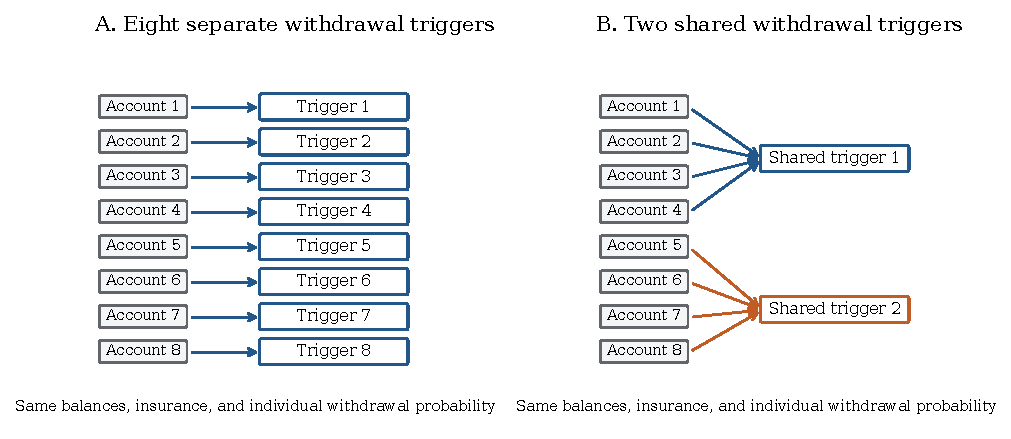
\includegraphics[width=\linewidth]{01-ownership-and-control.pdf}
\caption{Ownership and withdrawal control can differ. The two structures have identical account balances and individual withdrawal probabilities. Shared triggers alter joint cash demand. An economic controller is a common source of execution decisions; using the same software vendor alone does not establish common control.}
\label{fig:control}
\end{figure}

\section{Related literature and the scope of the contribution}
\paragraph{Deposits as a source of liquidity and franchise value.}
\citet{diamond1983} explain the liquidity services and fragility of demand deposits. \citet{kashyap2002} connect deposit-taking and lending through shared liquidity needs. Deposit market power and the value of sticky funding are central to \citet{drechsler2017}; \citet{drechsler2026} show how loss of the deposit franchise can itself create run incentives. We hold the withdrawal-response environment fixed and study a treasury problem within it. There is no sequential-service game, endogenous solvency signal, or equilibrium selection in our model.

\paragraph{Digital mobility and depositor characteristics.}
\citet{koont2024} study digital banking and deposit-franchise stability. \citet{brei2026} examine how digital banking and social media interact in deposit pricing. \citet{narayanan2024} connect depositor characteristics with deposit-rate setting and flows. These studies establish that deposit technology and customer composition affect funding. Our comparative statics instead hold marginal withdrawal incentives fixed while changing the distribution of control over accounts. This isolates a dependence channel from a change in average price sensitivity.

\paragraph{Financial agents and concentration.}
\citet{phillips2025} directly anticipates AI agents acting as deposit brokers and discusses coordinated withdrawals and supervisory authority. Supervisory guidance recognizes concentration and the volatility of some insured nontraditional deposits \citep{robinson2024}; liquidity standards also distinguish deposit categories and customer relationships \citep{basel2013}. We formalize a horizon-specific limit on balances subject to joint execution and quantify the funding-risk information that such a limit supplies.

\paragraph{Dependence, moments, and computation.}
Majorization and convex ordering provide the exposure comparison \citep{marshall2011}, while comonotonic aggregation provides the unrestricted-dependence benchmark \citep{dhaene2002}. \citet{scarf1958} establishes the classical distributionally robust inventory problem; \citet{bertsimas2005} develops moment-based probability bounds. Our common-state floor is a bounded-support stop-loss result in that tradition. The bank's objective has the expected-shortfall representation of \citet{rockafellar2002}. Polynomial bounds using Bernstein coefficients are also established \citep{bensassi2015}.

The closest statistical antecedents are bounds and representations for multivariate and exchangeable Bernoulli variables \citep{fontana2022,fontana2023}. Those works already show the importance of the assumed dependence class. Our finite-exchangeable sensitivity calculation is an application of that framework. The cap-based disclosure frontier additionally optimizes over unknown, unequal control exposures and connects the resulting uncertainty to a bank's funding choice.

Relative to these antecedents, the analysis links an incomplete disclosure of delegated withdrawal authority to an extremal exposure structure, a common-state limiting frontier, and endogenous liquidity choice. The public-data exercise then places that frontier on observed balance-sheet scales. The repository provides a detailed record of the literature reviewed through 23 September 2026.

\section{A bank with delegated deposit control}
\subsection{Balances, decisions, and the measurement horizon}
Fix a horizon over which a bank must meet withdrawals before it can costlessly adjust its asset portfolio. Let \(D>0\) be the amount of deposits potentially managed through the mechanism under study. A controller \(j\) governs balance \(Dw_j\), where
\begin{equation}
 w_j\geq0,\qquad \sum_{j=1}^{m}w_j=1.
 \label{eq:weights}
\end{equation}
An account can be divided into portions with different mandates. The weights describe jointly responsive balances, rather than the number of legal accounts, application downloads, or model vendors. A controller can be a shared execution rule even when legal ownership remains dispersed.

Let \(X_j\in\{0,1\}\) indicate an executed withdrawal of controller \(j\)'s balance during the horizon. Normalized withdrawals are
\begin{equation}
 W_w=\sum_{j=1}^m w_jX_j\in[0,1].
 \label{eq:W}
\end{equation}
For the reference model, a random common propensity \(P\in[0,1]\) governs conditionally independent triggers:
\begin{equation}
 (X_1,\ldots,X_m)\mid P=p\ \sim\ \bigotimes_{j=1}^m\operatorname{Bernoulli}(p).
 \label{eq:conditional}
\end{equation}
The common state can summarize a change in outside yields, shared news, or a common input to execution rules. The bank's cash decision is made before this state is realized. This is a reduced-form withdrawal model. It does not make \(P\) a measured feature of an LLM or assume that depositors literally randomize after receiving advice.

The all-or-nothing representation can also serve as an upper-bound construction. Suppose each controller instead withdraws \(Y_j\in[0,w_j]\), with \(\E[Y_j\mid P=p]=pw_j\), independently across controllers conditional on \(P\). A Bernoulli endpoint withdrawal with the same conditional mean is larger in convex order. Thus the bound below covers partial withdrawals satisfying these conditions; exact Bernoulli blocks attain it.

\subsection{Information and dependence}
The bank observes, or selects for stress testing,
\begin{equation}
 \E[P]=\mu,\qquad \E[P^2]=\nu
 =\mu^2+\rho\mu(1-\mu),\qquad 0<\mu<1,\quad0\leq\rho\leq1.
 \label{eq:moments}
\end{equation}
Under \eqref{eq:conditional}, each trigger has mean \(\mu\), and distinct triggers have correlation \(\rho\). Define the admissible common-state laws
\begin{equation}
 \G(\mu,\nu)=\{G:\operatorname{supp}(G)\subseteq[0,1],\
                   \textstyle\int p\,dG=\mu,\ \int p^2\,dG=\nu\}.
 \label{eq:G}
\end{equation}
If \(\rho=0\), \(P=\mu\) almost surely. If \(\rho=1\), \(P\) is supported on \(\{0,1\}\). For intermediate values, the first two moments do not determine \(G\).

A disclosure may further certify
\begin{equation}
 \max_jw_j\leq h,\qquad 0<h\leq1.
 \label{eq:cap}
\end{equation}
This is information about an existing control structure. An intervention that changes that structure is a separate economic decision. A lower reported cap must correspond to genuinely separate triggers; renaming accounts or dividing one controller into nominal subsidiaries does not establish it.

For reference, the withdrawal variance is
\begin{equation}
 \operatorname{Var}(W_w)=(\mu-\nu)\sum_jw_j^2+\nu-\mu^2.
 \label{eq:variance}
\end{equation}
The first term is controller-specific granularity; the second is common-state variation. Knowing this variance does not generally determine the expected funding shortage at a particular cash level.

\subsection{The bank's liquidity choice}
Let \(\ell\in[0,1]\) be cash allocated per unit of delegated balances. The bank incurs opportunity cost \(r\ell\) and incremental shortage cost \(c\E\pos{W_w-\ell}\), with \(0<r<c\). This gives
\begin{equation}
 C(w,G)=\min_{0\leq\ell\leq1}
 \left\{r\ell+c\E_G\pos{W_w-\ell}\right\}.
 \label{eq:cost}
\end{equation}
The monetary value is \(DC(w,G)\). One interpretation is a treasury with access to emergency funding whose incremental cost is locally linear. The same expression is a first-order approximation to costly asset liquidation. It does not model an unlimited capacity to sell assets at a fixed price, nor translate an uncovered withdrawal directly into bank failure.

An exogenous return on funds left outside cash makes \(D(1-\ell)\) a measure of the bank's chosen lending allocation in this partial-equilibrium problem. We do not endogenize loan demand, deposit-rate competition, emergency-funding prices, or the total deposit base. A higher minimized cost reduces the net funding value at given returns; its implication for lending requires separately examining the optimizer.

With only the cap and moments known, the bank evaluates
\begin{align}
 \U_h(\ell;\mu,\nu)
 &=\sup_{\substack{m\geq1,\ w\geq0,\ \sum w_j=1\\ \max w_j\leq h}}
       \sup_{G\in\G(\mu,\nu)}\E_G\pos{W_w-\ell},\label{eq:U}\\
 C_h(\mu,\nu)&=\min_{0\leq\ell\leq1}
       \{r\ell+c\U_h(\ell;\mu,\nu)\}.\label{eq:robustcost}
\end{align}
This is robust valuation conditional on a stated model class. It is not the prediction that an adversarial state distribution will occur.

\section{What ownership and marginal behavior do not identify}
\begin{proposition}[Ownership invariance and a funding-cost wedge]\label{prop:ownership}
Splitting or relabeling accounts without changing the controller balances leaves the law of \(W_w\) unchanged. Consider \(N\) equal accounts, each with withdrawal probability \(\mu\). If all accounts share one trigger, then
\(\E\pos{W-\ell}=\mu(1-\ell)\) and
\(C=\min\{r,c\mu\}\).
If their triggers are independent, then as \(N\to\infty\),
\(\E\pos{W-\ell}\to\pos{\mu-\ell}\) uniformly in \(\ell\), and \(C\to r\mu\).
The ratio of the two limiting costs is
\begin{equation}
 \frac{\min\{r,c\mu\}}{r\mu}=\min\{1/\mu,c/r\}.
 \label{eq:ratio}
\end{equation}
\end{proposition}
The two structures have the same legal account concentration, balance totals, and individual withdrawal probabilities. A controller disclosure distinguishes them. A disclosure of legal account count alone does not. Deposit insurance can change withdrawal incentives, hence \(\mu\), but it does not mechanically force different insured accounts to use independent execution rules.

More generally, any \(W\in[0,1]\) with mean \(\mu\) satisfies
\begin{equation}
 \pos{\mu-\ell}\leq\E\pos{W-\ell}\leq\mu(1-\ell).
 \label{eq:generic}
\end{equation}
The inequalities are Jensen's inequality and the chord bound for a convex function. They are classical. Their economic implication here is that an average runoff rate alone permits a large range of liquidity values. The next section shows exactly how a cap on delegated control narrows that range under \eqref{eq:conditional}.

\section{The control-disclosure frontier}
\subsection{A sharp extremal control structure}
Let \(q=\lfloor1/h\rfloor\), \(a=1-qh\), and define
\begin{equation}
 w^h=(\underbrace{h,\ldots,h}_{q\text{ entries}},a),
 \label{eq:extreme}
\end{equation}
omitting the last entry when \(a=0\). Its number of positive entries is \(m_h=\lceil1/h\rceil\).

\begin{theorem}[Sharp cap-based aggregation]\label{thm:cap}
For every finite control vector satisfying \eqref{eq:weights}--\eqref{eq:cap}, every common-state law \(G\), and every convex function \(\phi\),
\begin{equation}
 \E_G\phi(W_w)\leq\E_G\phi(W_{w^h}).
 \label{eq:convexorder}
\end{equation}
Consequently, writing \(g_h(p,\ell)=\E[\pos{W_{w^h}-\ell}\mid P=p]\),
\begin{equation}
 \U_h(\ell;\mu,\nu)=\max_{G\in\G(\mu,\nu)}\int g_h(p,\ell)\,dG(p).
 \label{eq:reduction}
\end{equation}
The same upper bound holds for conditionally independent partial withdrawals \(Y_j\in[0,w_j]\) with conditional means \(pw_j\). It is attained within that class by endpoint Bernoulli withdrawals and \(w^h\).
\end{theorem}
The proof applies the standard majorization order to conditional expected convex cost. The financial consequence is useful: the entire undisclosed control map can be replaced by a single explicit extremal map, provided the cap is credible and the dependence assumptions are maintained. The bank need not enumerate partitions of thousands of accounts.

The frontier is nondecreasing in \(h\), since a looser cap enlarges the admissible set. This is a statement about a maximum over possible control structures. It does not say that every vector with a larger maximum coordinate is more risky than every vector with a smaller one. Comparisons between two known vectors require a stronger ordering, such as majorization, or direct calculation.

\subsection{Polynomial representation and moment bounds}
Write \(B_{k,m}(p)=\binom{m}{k}p^k(1-p)^{m-k}\). Conditional on exactly \(k\) triggers among the \(m=m_h\) controllers, each subset of size \(k\) is equally likely. Thus
\begin{equation}
 g_h(p,\ell)=\sum_{k=0}^{m}\beta_k(\ell)B_{k,m}(p).
 \label{eq:bernstein}
\end{equation}
If \(a=0\), \(\beta_k(\ell)=\pos{k/m-\ell}\). Otherwise,
\begin{equation}
 \beta_k(\ell)=\frac{m-k}{m}\pos{kh-\ell}
 +\frac{k}{m}\pos{(k-1)h+a-\ell}.
 \label{eq:beta}
\end{equation}
This reduces exposure aggregation to \(m+1\) coefficients rather than \(2^m\) withdrawal configurations.

\begin{theorem}[Moment formulation and verifiable bounds]\label{thm:moments}
For \(\mu^2<\nu<\mu\), the maximum in \eqref{eq:reduction} is attained by a distribution on at most three points and equals
\begin{equation}
 \inf_{y\in\R^3}\left\{y_0+y_1\mu+y_2\nu:
 y_0+y_1p+y_2p^2\geq g_h(p,\ell)\quad\forall p\in[0,1]\right\}.
 \label{eq:dual}
\end{equation}
Let \(\widetilde\beta_{k,N}\) be the coefficients of \(g_h\) elevated to degree \(N\geq\max\{m,2\}\). Any \(y\) satisfying
\begin{equation}
 y_0+y_1\frac{k}{N}+y_2\frac{k(k-1)}{N(N-1)}
 \geq\widetilde\beta_{k,N},\qquad k=0,\ldots,N,
 \label{eq:bernconstraint}
\end{equation}
provides an upper bound in \eqref{eq:dual}. Any distribution on a finite grid with the required moments provides a lower bound. The Bernstein upper bounds converge to \(\U_h\) as \(N\to\infty\).
\end{theorem}
The support and dual statements are specializations of the classical moment problem \citep{bertsimas2005}. The Bernstein inequalities are sufficient for global polynomial domination, not merely domination at sampled points. Degree elevation tightens the sufficient condition. A grid-only evaluation of a candidate majorant would not establish an upper bound between grid points.

The endpoint moment cases require no optimization: \(\rho=0\) fixes \(P=\mu\); \(\rho=1\) fixes masses \(1-\mu,\mu\) at \(0,1\). The implementation handles both analytically. At any cap with at most two positive extremal blocks, \(g_h\) is quadratic, so the first two common-state moments determine its expectation exactly. With three or more blocks, higher moments can matter.

\subsection{A common-state floor}
Let
\begin{equation}
 \U_0(\ell;\mu,\nu)=\max_{G\in\G(\mu,\nu)}\E_G\pos{P-\ell},\qquad
 \sigma^2=\nu-\mu^2.
 \label{eq:floor}
\end{equation}
This is the residual risk in the infinitely dispersed-control limit.

\begin{theorem}[Uniform floor and diversification limit]\label{thm:floor}
For every cap \(h\) and cash level \(\ell\),
\begin{equation}
 0\leq\U_h(\ell;\mu,\nu)-\U_0(\ell;\mu,\nu)
 \leq\frac12\sqrt{h(\mu-\nu)}.
 \label{eq:floorbound}
\end{equation}
For \(\sigma^2>0\), define
\(t_-=\nu/(2\mu)\) and \(t_+=(1-\nu)/(2(1-\mu))\). The sharp bounded-support floor is
\begin{equation}
 \U_0(\ell)=
 \begin{cases}
 \mu-\ell\mu^2/\nu,&0\leq\ell<t_-,\\[2pt]
 \tfrac12\!\left[\sqrt{(\ell-\mu)^2+\sigma^2}+\mu-\ell\right],
       &t_-\leq\ell\leq t_+,\\[2pt]
 (1-\ell)\sigma^2/(1-2\mu+\nu),&t_+<\ell\leq1.
 \end{cases}
 \label{eq:floorformula}
\end{equation}
When \(\sigma^2=0\), \(\U_0(\ell)=\pos{\mu-\ell}\).
\end{theorem}
Equation~\eqref{eq:floorformula} is the bounded-support version of a classical two-moment stop-loss bound; we provide the extremal laws and a proof for completeness. The application-specific statement is the uniform connection from this floor to every admissible finite control structure.

Under independent triggers and \(\ell>\mu\), the residual shortage vanishes rapidly as \(h\) shrinks. With a nondegenerate common propensity, the worst-case floor remains strictly positive for \(\ell<1\). More accounts or more separate controllers cannot remove this component. A policy aimed at controller granularity and one aimed at common incentives therefore address different sources of funding risk.

\begin{figure}[t]
\centering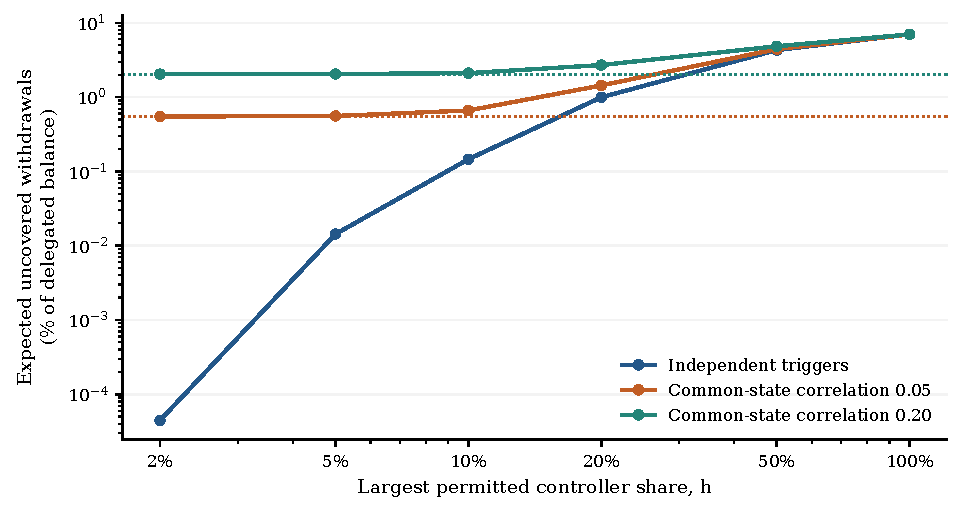
\includegraphics[width=\linewidth]{02-control-and-common-risk.pdf}
\caption{The cap-based frontier and its common-state floor. Mean trigger probability is 0.10 and cash is 0.30 of delegated balances. Curves report the worst admissible common-state law at each cap; shaded bands are numerical lower--upper brackets and dotted lines are the analytical floors. Both axes use logarithmic scales. The independent case is calculated exactly from binomial probabilities.}
\label{fig:frontier}
\end{figure}

\section{Funding value, lending, and the price of information}
\subsection{Robust liquidity choice}
Define \(\alpha=r/c\in(0,1)\). For a known withdrawal law, the minimizing cash levels satisfy
\begin{equation}
 \Pp(W>\ell)\leq\alpha\leq\Pp(W\geq\ell).
 \label{eq:quantile}
\end{equation}
Using the expected-shortfall convention that averages the upper \(\alpha\) fraction of the distribution, including a fractional atom when needed,
\begin{equation}
 C(w,G)=r\,\ES_{1-\alpha}(W_w).
 \label{eq:ES}
\end{equation}
This is the representation of \citet{rockafellar2002}, applied to withdrawal demand rather than a portfolio loss.

\begin{proposition}[Funding value under control disclosure]\label{prop:choice}
The robust cost satisfies
\begin{equation}
 C_h=r\sup_{G\in\G(\mu,\nu)}\ES_{1-\alpha}(W_{w^h}).
 \label{eq:robustES}
\end{equation}
It is nondecreasing in \(h\). If \(C_0=\min_\ell\{r\ell+c\U_0(\ell)\}\), then
\begin{equation}
 0\leq C_h-C_0\leq\frac{c}{2}\sqrt{h(\mu-\nu)}.
 \label{eq:costfloor}
\end{equation}
For a known law, a mean-preserving concentration of control increases minimized funding cost, but need not increase optimal cash.
\end{proposition}
The minimax equality follows from convexity in cash, linearity in the common-state law, and compactness \citep{sion1958}. It allows a single law to certify a lower bound on the bank's optimized robust cost. A lower bound evaluated only at the bank's candidate cash choice would not serve this purpose, since another cash choice might be cheaper.

For the cash comparison, consider independent triggers with \(\mu<\alpha\). Under one controller, the optimum is \(\ell=0\): cash costs more at the margin than it saves in the infrequent withdrawal event. Under a sufficiently dispersed structure, the optimum approaches \(\mu\). Concentrating control thus raises cost from approximately \(r\mu\) to \(c\mu\) while raising the allocation \(1-\ell\) to lending. In the finite reference calculation, changing the cap from 2 percent to 100 percent lowers selected cash from 14 percent to zero and raises normalized cost from 0.03237 to 0.10.

This result cautions against interpreting an increase in credit supply, by itself, as evidence that delegated funding is safer. It does not imply that banks should increase lending under concentrated control. The choice depends on the shortage price, liquidity constraints, and risk preferences omitted from this partial-equilibrium example. A sufficiently strong minimum-liquidity requirement would also alter it.

\subsection{Disclosure value versus an operational intervention}
Suppose an existing control structure is known only to satisfy cap \(h_2\). A credible audit establishes a tighter cap \(h_1<h_2\), without moving a single deposit. The reduction
\begin{equation}
 V(h_1,h_2)=D\,[C_{h_2}-C_{h_1}]\geq0
 \label{eq:informationvalue}
\end{equation}
is the reduction in this bank's robust funding-cost assessment. It is a model-based value of the additional information, not a realized cash saving or the welfare gain from breaking up a platform. An operational reorganization must additionally account for user benefits, implementation cost, execution quality, and any induced change in \(\mu\) or \(G\).

The floor provides a stopping criterion for ever finer granularity: if the cost of a further audit or reorganization exceeds the maximum remaining reduction permitted by \eqref{eq:costfloor}, granularity alone cannot justify that expenditure within the model. Better measurement or management of the common state may then be more valuable.

\subsection{Why correlation reporting is incomplete}
At \(\mu=0.10\), \(\rho=0.05\), one admissible law places mass at \(0\) and \(\nu/\mu=0.145\). Another, chosen at cash \(\ell=0.30\), places mass at
\(\ell\pm\sqrt{(\ell-\mu)^2+\sigma^2}\).
Both have the same first two moments. In the dispersed-control limit, the first law has zero shortage at this cash level; the second attains \eqref{eq:floorformula}. This is not a disagreement about estimation error. It is nonidentification of a nonlinear funding cost from the specified information.

For a fixed vector of \(m\) positive controller weights, the full law of \(W_w\) is determined by the first \(m\) moments of \(P\), and conversely determines those moments. The latter follows by expanding \(\E[W_w^k\mid P]\): the coefficient on \(P^k\) is \(k!e_k(w)>0\), where \(e_k\) is the elementary symmetric polynomial. The first \(m\) unconditional moments can therefore be inverted recursively. This is the familiar finite-mixture moment limitation in another form. Recording a variance does not generally replace information about higher-order co-withdrawal events.

\begin{figure}[t]
\centering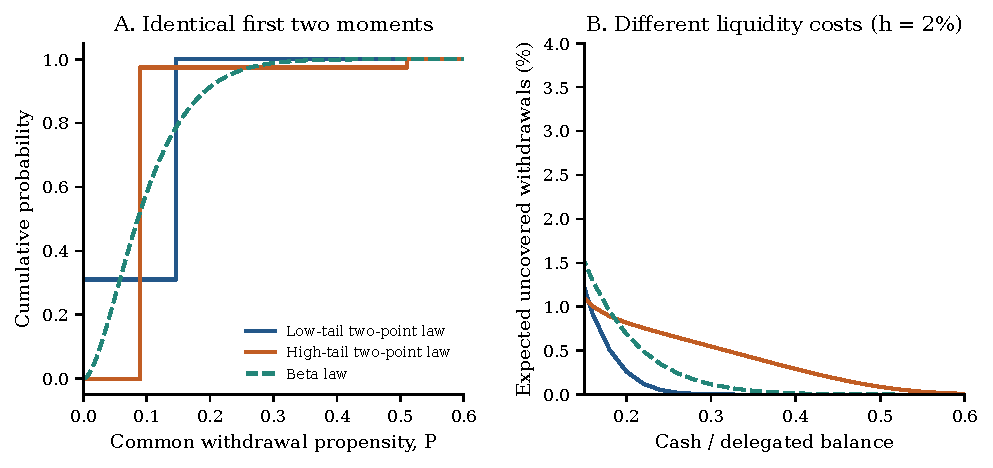
\includegraphics[width=\linewidth]{03-moments-and-tails.pdf}
\caption{Equal moments do not identify liquidity cost. All three common-state distributions have mean 0.10 and trigger correlation 0.05. The two-point laws are fixed across the cash levels in panel B, which uses 50 equal control blocks. The high-tail law is extremal for the common-state limit at cash 0.30; it is not asserted to maximize every finite-block calculation or every cash level.}
\label{fig:moments}
\end{figure}

\section{Computation and controlled quantitative results}
\subsection{Reproducible design}
The local protocol preceded the numerical experiments; it is preserved with a hash. The fixed-cash sweep comprises 270 cases: three mean probabilities, five correlations, six caps, and three cash levels. The bank-choice sweep contains 90 combinations of correlation, cap, and cost ratio. A further 3,618 evaluations construct cash frontiers for the figures and balance-sheet illustration. These are deterministic evaluations of stated scenarios, not independent observations from an economic population.

The initial upper calculations use Bernstein degree 512; the lower moment problems use a 1,001-point uniform grid augmented by \(\mu\), \(\nu/\mu\), and \((\mu-\nu)/(1-\mu)\). These additional nodes keep simple extremal moment laws feasible. We then refine the 18 central fixed-cash cases through degrees 1,024, 2,048, and 4,096 with a 4,001-point grid. The 18 corresponding cash-choice cases are also refined to degree 4,096. Refinement was prompted by visible numerical gaps and is documented separately from the original protocol.

The upper-bound problem is a three-variable linear program at fixed cash. The bank-choice problem jointly selects cash, positive-part epigraphs at feasible withdrawal amounts, and a polynomial majorant. Its lower program selects a grid-supported common-state distribution and maximizes the bank's minimum cost. The supremum over state laws can bend between withdrawal amounts, so restricting the robust bank's cash choice to those amounts is generally invalid. The implementation permits interior solutions.

\subsection{The effect of control granularity}
Table~\ref{tab:risk} holds \(\mu=0.10\) and \(\ell=0.30\) fixed. The independent column uses \(\rho=0\). The beta and moment-robust columns both use \(\rho=0.05\), with beta parameters \(\mu(1/\rho-1)\) and \((1-\mu)(1/\rho-1)\).

\begin{table}[t]
\centering\small
\caption{Expected uncovered withdrawals under alternative information}
\label{tab:risk}
\begin{tabular}{rrrrrr}
\toprule
Cap & Independent & Beta & Robust lower & Robust upper & Gap (bp)\\
\midrule
\inputrows{table-risk.tex}
\bottomrule
\end{tabular}
\begin{minipage}{\linewidth}\footnotesize\vspace{3pt}
Notes: Loss columns are percentages of delegated balances; the gap is in basis points of delegated balances. Mean withdrawal probability is 0.10 and cash is 0.30. The beta and robust cases share correlation 0.05. Independent triggers have correlation zero. Upper bounds use degree 4,096; lower bounds are feasible common-state laws.
\end{minipage}
\end{table}

At a 20-percent cap, the beta calculation is close to the moment bound. At a two-percent cap, it is less than one quarter of the worst admissible value. This difference reflects the shape of the common-state distribution. A beta specification is not uniformly conservative merely because it matches the observed mean and correlation.

The independent calculation at a two-percent cap is very small, approximately \(4.45\times10^{-7}\) of delegated balances. The common-state floor at correlation 0.05 is approximately 0.005475. The large ratio between these values is a consequence of the maintained dependence scenarios, not an empirical estimate of an AI effect. At correlation one, all caps give the same expected shortage \(\mu(1-\ell)\): granularity has no value.

\subsection{Endogenous cash and the common-state floor}
Figure~\ref{fig:choice} reports the bank's chosen cash and minimized cost when \(r/c=0.20\). At correlation 0.05, reducing the cap from 100 percent to two percent lowers normalized robust cost from 0.10 to a bracket of approximately 0.047456--0.047494. The chosen cash at the smaller cap is about 0.157. The infinitely dispersed-control cost is 0.046833, so most of the residual value is limited by common-state risk.

For an interior optimum in the middle branch of \eqref{eq:floorformula}, direct minimization gives
\begin{equation}
 \ell_0=\mu+\frac{\sigma(1-2\alpha)}{2\sqrt{\alpha(1-\alpha)}},\qquad
 C_0/c=\alpha\mu+\sigma\sqrt{\alpha(1-\alpha)}.
 \label{eq:floorchoice}
\end{equation}
The branch and unit-interval conditions must be checked before applying this expression. They hold in the reference example. Outside this region, the optimizer can lie on a boundary or in a linear branch.

\begin{figure}[t]
\centering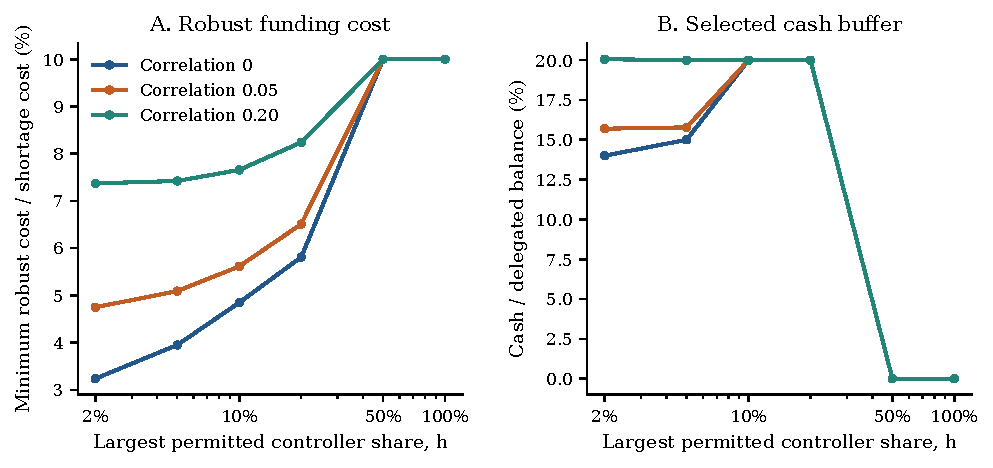
\includegraphics[width=\linewidth]{04-bank-choice.pdf}
\caption{Funding costs and cash choices are different comparative statics. Mean trigger probability is 0.10 and the opportunity-cost/shortage-cost ratio is 0.20. Panel A reports valid upper costs, with numerical optimization gaps below 0.000038 in the refined cases. Panel B reports a minimizing cash choice for the finite upper program; at ties, the implementation may select one of several minimizers. Lines connect discrete cap scenarios.}
\label{fig:choice}
\end{figure}

\subsection{Sensitivity to the dependence class}
Conditional independence given a common propensity is stronger than finite exchangeability. To measure that restriction, consider \(n=1/h\) equal control blocks and let \(K\) be their number of withdrawals. Any exchangeable law is described by probabilities \(z_k=\Pp(K=k)\). Keeping the same marginal probability and pairwise correlation imposes
\begin{equation}
 \sum_kz_k=1,\quad \sum_kkz_k=n\mu,\quad
 \sum_kk(k-1)z_k=n(n-1)\nu,\quad z_k\geq0.
 \label{eq:finiteexchange}
\end{equation}
Maximizing \(\sum_kz_k\pos{k/n-\ell}\) is a finite linear program \citep{fontana2022,fontana2023}.

\begin{table}[t]
\centering\small
\caption{The maintained dependence class materially affects the bound}
\label{tab:assumptions}
\begin{tabular}{rrr}
\toprule
Cap (\%) & Conditional-mixture bracket (\%) & Finite-exchangeable maximum (\%)\\
\midrule\inputrows{table-assumptions.tex}\bottomrule
\end{tabular}
\begin{minipage}{\linewidth}\footnotesize\vspace{3pt}
Notes: Equal blocks with \(n=1/h\), mean 0.10, correlation 0.05, and cash 0.30. The finite-exchangeable class contains the conditional-mixture class. This comparison changes the dependence assumption, not the reported marginal or pairwise moments.
\end{minipage}
\end{table}

At a ten-percent cap, the broader maximum is 1.305 percent, compared with approximately 0.661--0.662 percent under the conditional-mixture model. The tighter bound therefore cannot be justified from pairwise correlation alone. With no restriction on dependence or its moments beyond a common marginal probability, all triggers may coincide and even an arbitrarily small controller cap permits the upper bound in \eqref{eq:generic}. Controller disclosure and dependence information are complementary.

\subsection{Numerical verification}
The code checks conditional-count coefficients against exhaustive enumeration, degree elevation against direct polynomial evaluation, and the moment programs against known limiting cases. Tests also cover partial refinements of control blocks, probability-mass conservation, global polynomial domination, and the distinction between cash and funding cost.

For the 18 refined fixed-cash cases, a separate exact-arithmetic routine converts the proposed quadratic coefficients to rational numbers, checks every degree-4,096 Bernstein inequality with integer arithmetic, and repairs the constant coefficient upward if needed. It reconstructs rational probabilities on two or three support points and verifies the moment equalities exactly. Thus those reported certificates do not rely on the solver's floating-point feasibility flag. The broader parameter sweeps and bank-choice programs use numerical residual checks and explicit gaps; we do not describe them as interval-certified computations.

Six independent simulation checks each draw one million common states and conditional binomial counts. The largest absolute discrepancy between a Monte Carlo average and its analytical target is 1.83 estimated standard errors. For the smallest independent-tail case, simulation alone would be inefficient; the exact binomial calculation remains the primary result. The degree-4,096 fixed-cash gaps are below 0.000027, and refined bank-choice gaps are below 0.000038. These are numerical tolerances on normalized losses, not confidence intervals for economic parameters.

\begin{figure}[t]
\centering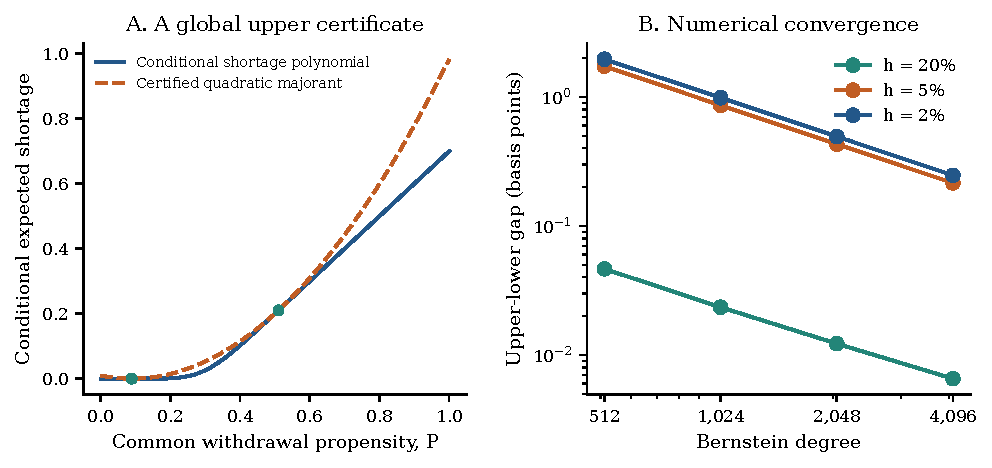
\includegraphics[width=\linewidth]{06-verification.pdf}
\caption{A verifiable computation. Panel A shows the conditional-loss polynomial and a globally dominating quadratic at \(h=0.02\), \(\mu=0.10\), \(\rho=0.05\), and \(\ell=0.30\). Points identify a feasible extremal-grid law. Global domination is checked through exact Bernstein coefficients, not inferred from the plotted grid. Panel B shows decreasing lower--upper gaps as polynomial degree rises.}
\label{fig:verification}
\end{figure}

\section{Public bank balance sheets: a disclosure illustration}
\subsection{Sample and variables}
We retrieve unmodified financial responses and field definitions from the FDIC BankFind API \citep{fdic2026}. The main date, 31 December 2025, was selected as a completed calendar year before computing balance-sheet scenarios. The endpoint returns 4,411 records. We exclude 73 records that are either noninsured institutions or insured foreign branches, then two records with nonpositive domestic deposits. The resulting 4,336 banks and savings institutions have positive assets and domestic deposits and nonnegative reported cash and balances due. Duplicate certificate numbers are checked before merging insurance flags.

All balance fields are reported in thousands of U.S. dollars. Domestic deposits are \texttt{DEPDOM}; total assets are \texttt{ASSET}. The primary buffer is \texttt{CHBAL}, cash and balances due from depository institutions. A sensitivity calculation adds \texttt{SCUST}, U.S. Treasury securities. These quantities are accounting measures. They do not establish unencumbered, immediately transferable cash, intraday availability, or regulatory high-quality liquid assets. Adding Treasury securities at reported value does not impose a stressed liquidation haircut. Conversely, the primary buffer omits other securities, borrowing capacity, and incoming payments.

Table~\ref{tab:data} reports sample composition. Bank size is measured by assets, with boundaries at \$1 billion, \$10 billion, and \$100 billion; each boundary belongs to the higher category. These are cross-sectional descriptions rather than treatment groups. The two supplementary snapshots, at year-end 2022 and 2024, are repeated cross sections rather than a balanced panel.

\begin{table}[t]
\centering\small
\caption{Year-end 2025 balance-sheet sample}
\label{tab:data}
\begin{tabular}{lrrrrr}
\toprule
Asset size & Banks & Deposits (\$tn) & Median cash (\%) & P10 (\%) & P90 (\%)\\
\midrule\inputrows{table-data.tex}\bottomrule
\end{tabular}
\begin{minipage}{\linewidth}\footnotesize\vspace{3pt}
Notes: Cash denotes \texttt{CHBAL}/\texttt{DEPDOM}. Quantiles give each bank equal weight. Deposits are domestic-office deposits. Source: archived FDIC BankFind financials and insurance flags.
\end{minipage}
\end{table}

\subsection{Mapping the frontier into bank units}
For bank \(i\), let \(T_i\) denote domestic deposits and \(B_i\) its selected buffer. Set a hypothetical potentially delegated pool \(D_i=\theta T_i\), with \(\theta\in\{0.10,0.25,0.50\}\). For each cap \(h\), its incremental expected uncovered withdrawal envelope is
\begin{equation}
 Q_i(h,\theta)=D_i\,\U_h\!\left(\min\{B_i/D_i,1\};0.10,0.0145\right).
 \label{eq:bankmap}
\end{equation}
The moment value 0.0145 corresponds to \(\mu=0.10\) and \(\rho=0.05\). The delegated share, controller cap, and common-state moments are scenario inputs; none is inferred from the bank data. The identity of the potentially movable accounts is unobserved. Because domestic deposits include time deposits, interpreting \(\theta\) as an executable mandate requires separate information on contractual access.

The full buffer is allocated to this incremental pool, while other outflows are held at zero. Equation~\eqref{eq:bankmap} therefore isolates a mechanism and cannot be interpreted as total funding needs. Inflows, central-bank access, interbank redistribution, loan commitments, and other withdrawals would require a fuller treasury model.

For computational efficiency, we evaluate fixed-cash envelopes on a 201-point grid. A chord between valid upper bounds remains an upper bound because \(\U_h\) is convex in cash. Lower bounds evaluate feasible common-state laws from the adjacent grid points at the bank's actual cash ratio. Interpolating lower-bound values themselves would not be valid. The reported interval includes this interpolation gap.

\begin{figure}[t]
\centering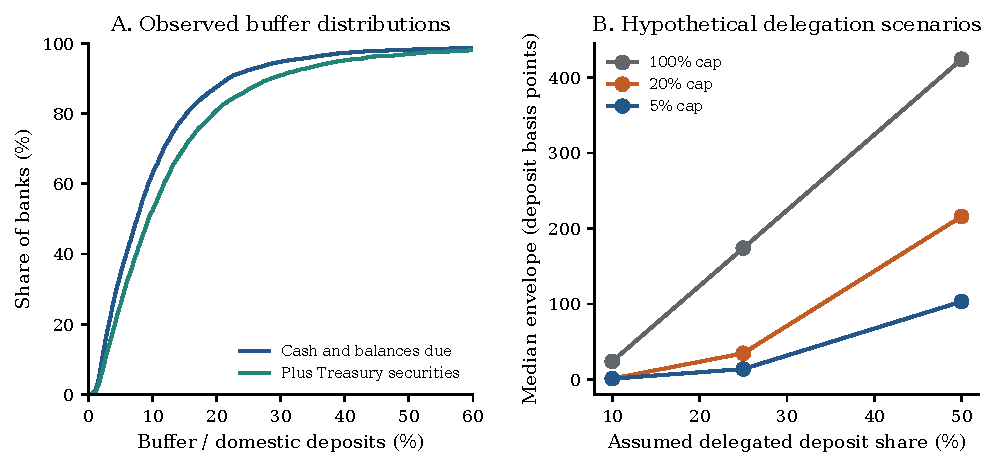
\includegraphics[width=\linewidth]{05-public-balance-sheets.pdf}
\caption{Public balance sheets supply scale, not a measure of delegated control. Panel A shows empirical buffer distributions across 4,336 banks at year-end 2025. Panel B reports median bankwise upper envelopes from hypothetical delegated shares and caps, holding the common-state moments fixed. The vertical units in panel B are basis points of each bank's domestic deposits. No plotted quantity estimates AI adoption or realized losses.}
\label{fig:banks}
\end{figure}

\subsection{What the illustration establishes}
At \(\theta=0.25\), the median bank's moment-robust cash-only envelope is 174.16 basis points of domestic deposits with one possible common controller. Under a five-percent cap, the median lies between 13.72 and 14.15 basis points. This difference quantifies what the two hypothetical control disclosures permit the analyst to rule out. It does not show that either structure currently describes the sampled banks.

\begin{table}[t]
\centering\small
\caption{Hypothetical delegation scenarios on 2025 balance sheets}
\label{tab:scenarios}
\begin{tabular}{rrrrr}
\toprule
Delegated share (\%) & Cap (\%) & Median bracket (bp) & Weighted upper (bp) & Max. gap (bp)\\
\midrule\inputrows{table-scenarios.tex}\bottomrule
\end{tabular}
\begin{minipage}{\linewidth}\footnotesize\vspace{3pt}
Notes: All basis points use domestic deposits as denominator. The weighted upper is \(10^4\sum_iQ_i^{\rm upper}/\sum_iT_i\), a deposit-weighted average of bankwise worst-case envelopes. Different banks' worst-case common-state laws need not coincide; this is not an identified systemwide event. The maximum gap includes finite-degree and interpolation error. Buffers are cash and balances due; mean and correlation are fixed at 0.10 and 0.05.
\end{minipage}
\end{table}

Adding Treasury securities lowers the median five-percent-cap bracket to 10.12--10.49 basis points at the same delegated share. The supplementary dates yield different levels as observed balance sheets change (Appendix~\ref{app:data}). None of these repeated-cross-section differences identifies an effect of delegation. They demonstrate why a universal account-based multiplier would miss bank-specific funding capacity even if the control parameters were known.

The data exercise also makes the principal measurement gap concrete. Public reports provide deposit totals and some ownership- and product-based categories. They do not identify the joint execution map assumed in \eqref{eq:weights}. Estimating that map, rather than labeling generic digital-bank activity as AI adoption, is the required next empirical step.

\section{Implementation and commercial interpretation}
A practical implementation would combine three records. First, a bank or aggregator would identify the amount an execution mandate can move over a specified horizon. Second, it would group mandates by economically shared triggers, including shared rules and delegated subcontrollers where those can jointly initiate transfers. Third, it would record the assumptions or evidence used for cross-controller dependence. The resulting withdrawal-control exposure record supplies \(D\), the control shares or their cap, and a scenario set for common-state moments.

The accompanying implementation accepts normalized exposures and explicit scenario parameters, returns cash-cost frontiers and feasible adversarial state laws, and exports polynomial certificates. Its commercial use would be in bank treasury scenario analysis, funding-transfer pricing, or an audit service for delegated account platforms. An aggregate cap can be reported without publishing each customer's balance. The method itself is not a cryptographic privacy guarantee, an automatic inference of hidden control relationships, or a validated production risk model.

Several operational distinctions are essential. A common LLM vendor is not necessarily a common withdrawal controller. Conversely, distinct vendors can implement the same trigger and remain economically synchronized. A controller's nominal size is not necessarily the balance movable within a short horizon. A customer's revocation right or manual override can change exposure. The record therefore needs an effective date, horizon, authority scope, and treatment of correlated fallback rules. Software diversity by itself does not certify the cap.

The model supports a comparison of voluntary mandate designs. Splitting control or staggering discretionary execution can impose opportunity costs on customers and may change average switching incentives. The cost reduction in \eqref{eq:informationvalue} is one input to that comparison; a welfare assessment must also value the customer's lost mobility and any change in service quality.

\section{Limits and empirical implications}
The withdrawal propensities in the quantitative exercises are stated inputs. Estimating them would require repeated observations at the controller and horizon level, a defensible definition of a common state, and treatment of regime changes. Confidence regions for moments could be incorporated by maximizing the dual objective over the region, but no such region is estimated here. The public balance sheets do not supply it.

The maintained conditional-independence structure is consequential, as Table~\ref{tab:assumptions} shows. Controllers with heterogeneous conditional probabilities, negatively dependent mandates, common technical failures outside \(P\), or endogenous responses to bank liquidity need a richer class. Subdividing a single trigger into nominally distinct controllers would invalidate a claimed cap benefit. These limitations are properties of the model, not small-sample qualifications that more simulation can remove.

The bank's cost function is also deliberately local. Convex external funding prices, a binding borrowing limit, simultaneous loan commitments, and endogenous fire-sale spillovers can alter optimal cash. The ordering in Theorem~\ref{thm:cap} survives replacing the positive-part loss by any convex funding-cost function, holding the environment fixed. The closed-form floor and the simple three-variable dual need not survive unchanged. Cross-bank allocation of a common controller's balances adds a network question that bankwise bounds alone do not answer.

The framework generates testable implications rather than a completed causal test. Holding conditional marginal withdrawal behavior fixed, an exogenous merger of execution triggers should increase convex funding costs. A genuine separation of triggers should reduce the idiosyncratic component in \eqref{eq:variance} while leaving the common component unchanged. Higher lending need not imply lower cost. A credible empirical design would need controller-level authority changes that are plausibly separate from customer selection, product repricing, and changing bank fundamentals. Those data would materially strengthen the link to observed financial intermediation.

\section{Conclusion}
Delegated deposit management makes authority over withdrawals a distinct characteristic of bank funding. Under a stated conditional-dependence model, a cap on jointly controlled balances yields a sharp exposure structure and a tractable liquidity-cost frontier. The resulting decomposition separates what finer control granularity can diversify from what common-state uncertainty preserves. It also separates a bank's funding value from its chosen lending allocation.

The practical result is an auditable disclosure-to-valuation method, accompanied by proofs, exact and numerical checks, and a public-balance-sheet illustration. Its next empirical requirement is specific: observe the authority to execute withdrawals and its dependence across controllers. Account ownership and a generic AI-adoption indicator cannot substitute for that information.

\FloatBarrier
\bibliographystyle{plainnat}
\bibliography{references}
\clearpage
\appendix
\section{Proofs and additional derivations}
\subsection{Proof of Proposition~\ref{prop:ownership}}
The expression in \eqref{eq:W} depends on accounts only through total balances assigned to each controller. Hence splitting an account without changing that assignment leaves withdrawals unchanged. A single trigger gives \(W=X\), so \(\E\pos{W-\ell}=\mu(1-\ell)\). The cost is linear in \(\ell\), attaining its minimum at zero if \(c\mu<r\), at one if \(c\mu>r\), and everywhere if equality holds.

With \(N\) independent equal triggers, \(\E W=\mu\) and \(\operatorname{Var}(W)=\mu(1-\mu)/N\). The positive-part function is one-Lipschitz, so
\[\sup_{\ell\in[0,1]}\left|\E\pos{W-\ell}-\pos{\mu-\ell}\right|
 \leq\E|W-\mu|\leq\sqrt{\mu(1-\mu)/N}.\]
Uniform convergence permits minimizing the limiting cost. Since \(c>r\), \(r\ell+c\pos{\mu-\ell}\) is minimized at \(\ell=\mu\), with value \(r\mu\). Division yields \eqref{eq:ratio}. \hfill\(\square\)

\subsection{Proof of Theorem~\ref{thm:cap}}
Fix \(p\), pad weight vectors with zeros to a common dimension, and define
\(F_p(w)=\E[\phi(\sum_jw_jX_j)\mid P=p]\).
For every realization of the trigger vector, the function of \(w\) inside this expectation is convex. Thus \(F_p\) is convex. Conditional exchangeability makes it symmetric. A symmetric convex function is Schur-convex \citep{marshall2011}.

Sort any feasible vector decreasingly. Its first \(k\) entries sum to at most \(\min\{kh,1\}\). The sorted vector \(w^h\) achieves this upper partial sum at every \(k\) before total mass is exhausted. Therefore \(w^h\) majorizes \(w\), proving \(F_p(w)\leq F_p(w^h)\). Integration over any \(G\) proves \eqref{eq:convexorder}. The extremal vector is feasible, so taking suprema gives equality in \eqref{eq:reduction}.

For partial withdrawals, condition on \(P=p\) and all coordinates except \(Y_j\). Convexity gives the chord inequality
\[\phi(s+Y_j)\leq(1-Y_j/w_j)\phi(s)+(Y_j/w_j)\phi(s+w_j).\]
Conditional independence and \(\E Y_j=pw_j\) show that replacing \(Y_j\) by a Bernoulli endpoint amount does not decrease expected convex cost. Repeat over positive coordinates and apply the preceding comparison. Zero weights can be omitted. \hfill\(\square\)

\subsection{Proof of Theorem~\ref{thm:moments}}
The set of probability measures on the compact interval is weakly compact. Its moment restrictions are weakly closed, so \(\G\) is compact and nonempty. Since \(g_h\) is continuous, a maximum is attained. A linear objective over this moment set has an extremal maximizer supported on at most three points: if more than three disjoint support pieces carry mass, their vectors of zeroth, first, and second moments are linearly dependent, permitting a nonzero signed perturbation that preserves all three restrictions. Such a measure is not extreme. The standard compact moment duality theorem yields \eqref{eq:dual} for interior moment vectors \citep{bertsimas2005}.

For a polynomial expressed in degree-\(N\) Bernstein form, its value is a convex combination of its coefficients because \(B_{k,N}(p)\geq0\) and \(\sum_kB_{k,N}(p)=1\). The degree-\(N\) coefficients of \(1,p,p^2\) are, respectively, \(1,k/N,k(k-1)/(N(N-1))\). Therefore \eqref{eq:bernconstraint} implies global domination. Its expected value is the stated dual objective. A feasible discrete law provides the opposite bound by direct integration.

For convergence, take an arbitrarily near-optimal polynomial majorant \(q\) and add a constant \(\varepsilon>0\). The polynomial \(q+\varepsilon-g_h\) is strictly positive on the compact interval. Its degree-elevated Bernstein coefficients converge uniformly to its values at \(k/N\), hence are positive for sufficiently large \(N\). Thus a feasible coefficient majorant exists within \(\varepsilon\), plus the original near-optimality error, of the exact optimum. Weak duality supplies the lower limit. \hfill\(\square\)

The elevation identity used in the code is
\begin{equation}
 \widetilde\beta_{k,N}=\sum_{j=\max(0,k-N+m)}^{\min(m,k)}
 \beta_j\frac{\binom{k}{j}\binom{N-k}{m-j}}{\binom{N}{m}}.
 \label{eq:elevation}
\end{equation}
The coefficients are hypergeometric probabilities. This form avoids large factorials in numerical computation and is also convenient for exact rational checking.

\subsection{Proof of Theorem~\ref{thm:floor}}
Conditional Jensen gives \(g_w(p,\ell)\geq\pos{p-\ell}\). For the upper difference, use \(x_+=(x+|x|)/2\) and \(\E[W_w\mid p]=p\):
\begin{align*}
0\leq g_w(p,\ell)-\pos{p-\ell}
&=\tfrac12\{\E[|W_w-\ell|\mid p]-|p-\ell|\}\\
&\leq\tfrac12\E[|W_w-p|\mid p]
\leq\tfrac12\sqrt{p(1-p)\sum_jw_j^2}.
\end{align*}
Since \(\sum_jw_j^2\leq h\), integrating and applying Cauchy--Schwarz yields a bound of \(\tfrac12\sqrt{h(\mu-\nu)}\), uniform in \(G\) and \(\ell\). Taking maxima gives \eqref{eq:floorbound} and proves uniform convergence as \(h\downarrow0\).

For the sharp floor, let \(t=\ell\). If \(t<t_-\), take a law supported on \(0,b\), where \(b=\nu/\mu\), with mass \(\mu^2/\nu\) at \(b\). It has the required moments and loss \(\mu-t\mu^2/\nu\). The polynomial
\[q(p)=p-t(2p/b-p^2/b^2)\]
dominates \(\pos{p-t}\): it is nonnegative because \(2t\leq b\), and \(q(p)-(p-t)=t(p/b-1)^2\geq0\). Its expectation equals the exhibited loss.

In the middle interval, set \(d=\sqrt{(t-\mu)^2+\sigma^2}\). The support points \(t-d,t+d\) lie in \([0,1]\) exactly when \(t_-\leq t\leq t_+\). Assign masses \((t+d-\mu)/(2d)\) and \((\mu-t+d)/(2d)\), respectively. Their mean and variance are \(\mu,\sigma^2\). The resulting loss is \((d+\mu-t)/2\). For any admissible law,
\[\E\pos{P-t}=\tfrac12\{\mu-t+\E|P-t|\}
 \leq\tfrac12\{\mu-t+\sqrt{\E(P-t)^2}\},\]
which proves optimality.

For \(t>t_+\), reflect the lower-interval argument with \(1-P\). The extremal support is \(b,1\), with \(b=(\mu-\nu)/(1-\mu)\), and the mass at one is \(\sigma^2/(1-2\mu+\nu)\). Since \(t>b\), its loss is the final branch of \eqref{eq:floorformula}; the reflected polynomial gives the matching upper bound. The formulas agree at the junctions. Degenerate variance fixes \(P=\mu\). \hfill\(\square\)

\subsection{Proof of Proposition~\ref{prop:choice}}
For each \(G\), \(F(\ell,G)=r\ell+c\int g_h(p,\ell)dG\) is continuous and convex in \(\ell\), and continuous affine in \(G\). Both decision sets are compact and convex. Sion's minimax theorem permits exchanging the minimum and maximum. Applying the expected-shortfall representation inside gives \eqref{eq:robustES}. Monotonicity follows either from the nested cap sets or pointwise monotonicity of \(\U_h\). Taking minima in the two uniform inequalities from Theorem~\ref{thm:floor} proves \eqref{eq:costfloor}.

For known laws ordered in convex order, \(\E\pos{W-\ell}\) is ordered at every \(\ell\). Thus the minimized costs are ordered. Optimal cash is a quantile, and convex order does not generally order quantiles. The example after the proposition provides a constructive counterexample within this model. \hfill\(\square\)

\subsection{Variance and the information contained in withdrawal laws}
Conditional variance and total expectation give
\[\operatorname{Var}(W_w)=\E[P(1-P)]\sum_jw_j^2+\operatorname{Var}(P),\]
which is \eqref{eq:variance}. For \(k\leq m\), expand \((\sum_jw_jX_j)^k\) and collect terms by the number of distinct trigger indices. A term with \(s\) distinct indices has conditional expectation \(P^s\). Terms using \(k\) distinct indices have total coefficient \(k!e_k(w)>0\). Thus knowledge of the first \(k\) moments of \(W_w\), after lower moments of \(P\) have been recovered, identifies \(\E P^k\). Conversely, all probabilities of trigger configurations are polynomials of degree at most \(m\), so the first \(m\) moments of \(P\) determine the withdrawal law. This establishes the claimed finite information equivalence without identifying the entire mixing distribution.

\section{Algorithms, certification, and replication}\label{app:algorithm}
The fixed-cash lower program chooses nonnegative masses \(z_s\) on nodes \(p_s\), with \(\sum z_s=1\), \(\sum z_sp_s=\mu\), and \(\sum z_sp_s^2=\nu\), to maximize \(\sum z_sg_h(p_s,\ell)\). Its upper companion is \eqref{eq:bernconstraint}. Both problems must return feasible results; neither an optimizer status nor a sampled plot alone validates the bound.

For cash choice, let \(s_1,\ldots,s_J\) be the distinct possible withdrawals under \(w^h\). Introduce variables \(v_j\geq s_j-\ell\) and \(v_j\geq0\). Conditional-count probabilities linearly map \(v\) into Bernstein coefficients of the funding shortage. The upper linear program minimizes \(r\ell+c(y_0+y_1\mu+y_2\nu)\) subject to global coefficient domination and \(0\leq\ell\leq1\). For the lower program, maximize \(t\) over feasible grid masses subject to
\[t\leq r s_j+c\sum_sz_sg_h(p_s,s_j),\qquad j=1,\ldots,J.\]
For each fixed state law, the bank's cost is linear between adjacent \(s_j\), so these constraints bound its minimum exactly on that grid of state laws. They do not restrict the upper problem's cash optimizer.

The exact fixed-cash certificate stores rational quadratic coefficients, state support points, and probabilities. The verifier recomputes \eqref{eq:elevation}, tests every coefficient inequality, and checks nonnegative probabilities and exact zeroth, first, and second moments. If floating-point conversion makes a coefficient slightly negative, raising \(y_0\) by the largest exact violation restores a valid majorant. Lower-certificate probabilities are solved anew with rational arithmetic; they are not accepted from a floating residual tolerance.

The repository includes raw FDIC JSON responses, retrieval metadata and SHA-256 hashes, field definitions, processed samples, all result tables, plotting scripts, tests, and manuscript source. A locked Python environment and a single offline replication command regenerate the results without accessing an API. The data download is a separate command, so a future revision of FDIC data cannot silently alter the archived calculations. The simulations use seed 1720406; each reported draw count refers to actual executed samples.

\clearpage
\section{Sample construction and additional balance-sheet scenarios}\label{app:data}
\begin{table}[H]
\centering\small
\caption{Sample flow by reporting date}
\begin{tabular}{rrrrr}
\toprule
Date & API records & Insurance/class exclusions & Invalid balances & Retained\\
\midrule\inputrows{table-flow.tex}\bottomrule
\end{tabular}
\begin{minipage}{\linewidth}\footnotesize\vspace{3pt}
Notes: Insurance/class exclusions remove \texttt{INSFDIC}\(\neq1\) and foreign branches (\texttt{BKCLASS=OI}). All two-record balance exclusions at each date have nonpositive domestic deposits. Remaining cash and asset values satisfy the stated validity checks. Dates identify separate cross sections.
\end{minipage}
\end{table}

\begin{table}[H]
\centering\small
\caption{Date and buffer sensitivity at a 25-percent delegated share and a five-percent cap}
\begin{tabular}{llrr}
\toprule
Date & Buffer & Banks & Median bracket (deposit bp)\\
\midrule\inputrows{table-dates.tex}\bottomrule
\end{tabular}
\begin{minipage}{\linewidth}\footnotesize\vspace{3pt}
Notes: Common-state mean and trigger correlation remain 0.10 and 0.05. Cash is cash and balances due; Treasuries are included at reported values. Differences are descriptive scenario sensitivities, not causal estimates of technology adoption.
\end{minipage}
\end{table}

The public balance-sheet illustration does not require estimated insured deposits to equal domestic deposits minus estimated uninsured deposits. The reported fields have their own definitions and adjustments. Neither residual is used as a proxy for delegated control. This avoids introducing a fictitious control measure through an accounting subtraction.
\end{document}
